\documentclass[12pt]{article}

\input{setup}

% \addbibresource{tnd.bib}

\begin{document}
%TC:ignore
\begin{titlepage}
\title{Inferring infectiousness: a joint model of the within-host viral kinetics of SARS-CoV-2}
\author[1]{Christopher Boyer\thanks{email: \href{mailto:cboyer@hsph.harvard.edu}{cboyer@hsph.harvard.edu}}}
\author[1,2]{Marc Lipsitch}
\affil[1]{Department of Epidemiology, Harvard T.H. Chan School of Public Health, Boston, MA.}
\affil[2]{Department of Immunology and Infectious Diseases, Harvard T.H. Chan School of Public Health, Boston, MA.}
\date{\today}
\maketitle

\begin{abstract}
During an infectious disease outbreak, providing accurate answers to many policy questions about transmission requires a detailed model of the natural history of infectiousness. Unfortunately, direct measures of infectiousness are generally unavailable. Instead, we often rely on proxies of within-host viral kinetics such as symptoms or results from antigen and PCR tests or viral culture. However, these proxies vary in terms of the ease of collection, scalability, and their relationship to viral shedding and therefore underlying infectiousness. Here, we use data from four prospective, densely sampled cohorts with longitudinal data on multiple proxies of viral shedding for approximately 2,000 infections to develop a Bayesian joint model for the within-host viral kinetics of SARS-CoV-2 infection. Modeling the joint distribution allows us to infer the possible values of harder to measure proxies at any point during the infection based on all the available data. 
\noindent \\
\vspace{0in} \\
\noindent\textit{Keywords:} 
\bigskip
\end{abstract}
\setcounter{page}{0}
\thispagestyle{empty}
\end{titlepage}
\pagebreak \newpage
\spacingset{1.45} % DON'T change the spacing!
%\setstretch{1.5}
\section{Introduction} \label{sec:introduction}
Accurate information about the internal dynamics of infection within a host are crucial for informing effective public health policies during outbreaks. Chief among these are the infectious period \textemdash the period of time in which a host is able to transmit infection to another individual---  and an individual's infectiousness \textemdash the current probability of onward transmission given contact with another susceptible host. Both parameters are essential for shaping policy recommendations on managing illness and are also critical inputs for building accurate transmission models. However, direct measurement of infectiousness poses significant challenges. As a result, researchers often rely on proxies of viral shedding, such as self-reported symptoms, antigen and polymerase chain reaction (PCR) test results, or viral culture data, to estimate infectiousness.

These proxies vary widely in their ease of collection, scalability, and correlation with actual viral shedding. Symptom-based assessments are subjective and can be influenced by individual variability and reporting biases. Antigen tests offer rapid results but may lack sensitivity, especially in asymptomatic individuals or at different stages of infection. PCR tests are highly sensitive but can detect non-viable viral RNA, potentially overestimating the period of infectiousness. Viral culture is considered the gold standard for assessing infectivity but is labor-intensive and not feasible for large-scale or rapid assessments.

The reliance on single proxies or sparsely collected data can lead to incomplete or inaccurate representations of an individual's infectiousness over time. This limitation hampers our ability to answer critical policy questions, such as determining optimal isolation periods or prioritizing testing strategies. There is a clear need for a comprehensive approach that integrates multiple proxies to more accurately model within-host viral kinetics.

In this study, we address this gap by developing a Bayesian joint model for the within-host viral kinetics of SARS-CoV-2 infection. Utilizing data from four prospective, densely sampled cohorts comprising approximately 2,000 infections, we integrate longitudinal measurements of multiple proxies of viral shedding. The Bayesian framework allows us to account for the uncertainties inherent in each proxy and to model their joint distribution over the course of infection.

By modeling the joint distribution, we can infer the likely values of harder-to-measure proxies at any given point during the infection based on the available data. This approach enhances the granularity and accuracy of the viral kinetics profiles, providing a more detailed understanding of infectiousness dynamics. It also facilitates the estimation of unobserved or missing data points, which is particularly valuable in real-world settings where complete data collection is often impractical.

Our findings have significant implications for public health policy and infectious disease modeling. A more accurate representation of within-host viral kinetics can improve transmission models, leading to better-informed decisions regarding intervention strategies such as quarantine durations, contact tracing, and resource allocation. Furthermore, the methodological framework we present is adaptable and can be applied to other infectious diseases, enhancing its utility beyond SARS-CoV-2.

In the sections that follow, we detail the methods used to develop our Bayesian joint model, present the results of our analyses, and discuss the implications of our findings for both modeling efforts and public health policy. By integrating multiple proxies of viral shedding, we aim to provide a robust tool for improving our understanding of infectiousness and enhancing the effectiveness of outbreak response strategies.



\section{Proxies for infectiousness} \label{sec:proxies}
The transmission of a viral pathogen between humans is a complex biological process influenced not only by within-host dynamics of infection but also by a variety of other environmental and behavioral factors. Consequently, measurement and quantification of infectiousness is challenging as it is contingent upon multiple forces. Nonetheless, a key component of infectiousness is the amount of replication competent virus shed by an infected individual, which is more easily observable. Therefore, we focus on modeling viral shedding and assume it is largely synonymous with individual infectiousness, although our model could, in principle, be extended to include additional environmental and behavioral determinants of transmission.

There are several approaches to measuring or inferring viral shedding that vary in terms of their accuracy, ease of use,cost, and scalability. We review the most common below.

\subsection{Infectious virus}
%A necessary pre-requisite for onward transmission of viral infection is the presence of infectious (that is, replication competent) virus. 
The gold standard diagnostic approach to determining whether replication competent virus is present is recovery via cell culture. This is achieved by innoculating susceptible cell lines with clinical specimen and measuring cytopathic effects via light microscopy, with infection confirmed either via RT-PCR of the supernatant of infected cells or by immunostaining for viral proteins. In the case of SARS-CoV-2, several cell lines can be used for isolation including a line from African green monkey kidney cells (Vero E6) and human lines from colorectal adenocarcinoma cells (Caco-2), lung adenocarcinoma cells (A549), and hepatocellular carcinoma cells (Huh7). These lines typically express either angiotensin converting enzyme 2 (ACE2; the receptor required for virus entry) or transmembrane protease 2 (TMPRSS2; another receptor important for virus entry).

While simple culture provides a qualitative assessment of the presence of infectious virus in an innoculated specimen, other methods are available that directly quantify the number of infectious virions. To produce viral titres, the specimen is serially diluted and used for innoculation. In a focus-forming assay, a monolayer of cells is innoculated with the clinical specimen and the cells are fixed one day after infection and immunostained with virus-specific antibodies creating visible groups of infected cells (foci) that can be counted. In a plaque-forming assay, a monolayer of cells is innoculated and plates are fixed 2-3 days post-infection and then stained with crystal violet, forming plaques in the presence of infectious virus that can be counted. Finally, in a 
50\% tissue culture infectious dose (TCID$_{50}$), a monolayer is innoculated and at 

The advantages of viral culture assays are that they directly detect replication competent virus and therefore come the closest to measuring infectious viral shedding. The disadvantages are that cultures are time-consuming and require specially trained laboratory personnel to properly handle and store. Results can vary substantially across cell lines or laboratories. In the case of an emerging pathogen like SARS-CoV-2, cultures had to be performed under biosafety level 3 laboratory conditions. For these reasons, cultures are often expensive and not routinely performed in the clinical setting. Therefore high quality cultures collected longitudinally within the same infection are rare.

\subsection{Viral nucleic acids}
In the clinical setting, laboratory diagnosis of viral infection generally relies instead on demonstration of viral RNA via a virus-specific RT-PCR performed on the clinical specimen. The amount of viral RNA in the sample can be quantified by calibrating the cycle threshold (Ct) value, representing the number of amplification cycles necessary to detect a signal, to reference samples containing proscribed number of viral copies per milliliter or swab. Following previous literature, we refer to this measure of viral RNA concentration as viral load. The strong correlation between viral load and infectious virus leads to its utility as proxy for infectiousness.

RT-PCR is highly sensitive and specific, and thus the gold standard for clinical diagnosis, but it does not distinguish between replication competent and residual RNA. For determining individual infectiousness, this creates challenges particularly in the late stages of infection when destroyed or inactivated virus creates a surfeit of residual RNA leading to positive results even when virions are not themselves infectious. Unlike viral culture RT-PCR assays can be standardized and scaled for mass testing in laboratory settings. They are therefore more commonly used in research, including in longitudinal studies. However, outside certain mass testing, quarantining, or occupational health environments, repeated testing with RT-PCR in the community, as a means for individuals to monitor infectiousness, is not available.

\subsection{Viral antigens}
Diagnostics that can be used in a household or community setting are more restricted. However, since the COVID-19 pandemic, there has been a surge in availability of antigen-detecting rapid diagnostic tests. These tests detect viral proteins from lysed samples by forcing them across a lateral flow field containing conjugate antibody, hereafter referred to as a lateral flow device (LFD). For SARS-CoV-2 tests, the nucleocapsid proteins are typical target antigens of LFDs. In their basic form, LFDs provide a qualitative assessment of whether viral antigen is present but there is often no set procedure for quantifying the amount or concentration, although some studies have attempted to develop grading systems based on the intensity of the test line and a handful of companies offer digital lateral flow reader that provide quantitative results. 

The advantages of LFDs are their speed and simplicity, allowing them to be used at home for more biologically-informed and individualized screening and isolation decisions. Although they can be inaccurate relative to RT-PCR when used for clinical diagnosis, LFDs do correlate strongly with the presence of infectious virus. LFD results can vary by manufacturer, whether they were self-swabbed or taken by a professional, and the type of sample (nasal versus oral). There has also been considerable interest in whether performance may vary across variants. 

\subsection{Symptoms}

\section{The model} \label{sec:model}
We propose a generative model of within-host viral kinetics during an acute infection that can be linked, through an observational process, to multiple measures of viral shedding. Consider longitudinal observations from $i = 1, \ldots, N$ infected individuals at times $t = 1, \ldots, T$ since innoculation. The data are realizations $\{(V_{it}, R_{it}, Y_{it}, \mathbf{Z}_{it}, \mathbf{X}_i, S_{i})\}$ where $V_{it}$ is infectious virus, $R_{it}$ is viral RNA copies, $Y_{it}$ is an indicator of symptom onset, $\mathbf{Z}_{it}$ is a vector of observed test or biomarker measurements, $\mathbf{X}_i$ is a vector of individual covariates (e.g. sex, age, immune history), and $\mathbf{S}_i$ is a vector of test characteristics, such as swab type and gene target. The vector $\mathbf{Z}_{it}$ contains proxy measurements for viral shedding including as viral culture ($V^*_{it}$), RT-PCR ($R^*_{it}$), and lateral flow tests for viral antigens ($L^*_{it}$), such that $\mathbf{Z}_{it} = (V^*_{it}, R^*_{it}, L^*_{it})$. We use the superscript $*$ to denote observed rather than true value and, for notational convenience, hereafter we suppress the indexes $i$ for individuals. 

Our goal is to characterize the joint distribution, 
$$
f(V_t, R_t, Y_t, \mathbf{Z}_t | \mathbf{X}, t, S; \theta)
$$
defining the within-host trajectories of viral shedding and test or biomarker results over time, where $\theta$ is a vector of parameters (we use $\theta$ generically throughout to represent as yet to be defined model parameters). To specify the model, we factorize the joint distribution into a product of conditional distributions. A natural factorization is:
\begin{align*}
    f(&V_t, R_t, Y_t, \mathbf{Z}_t | \mathbf{X}, S, t; \theta) = \\ & \quad \underbrace{f(V_t | \mathbf{X}, t; \theta)}_{\shortstack{infectious \\ virus}} \times \underbrace{f(R_t | V_t, \mathbf{X}, t; \theta)}_{\shortstack{viral RNA}} \times \underbrace{f(Y_t | V_t, R_t, \mathbf{X}, t; \theta)}_{\shortstack{natural history \\ of symptoms}} \times \underbrace{f(\mathbf{Z}_t | V_t, R_t, Y_t, \mathbf{X}, t, S; \theta)}_{\shortstack{observation \\ model}}
\end{align*}
where the first term describes the trajectory of infectious virus over time, the second term describes the total concentration of viral RNA over time conditional on the amount of infectious virus, the third term describes the onset of symptoms conditional on the amount of infectious virus and viral RNA, and the fourth term relates these to observed biomarker values and test results.

We posit models for each of these components in turn below.

\subsection{Infectious virus}
A commonly used mechanistic model describing the dynamics of viral proliferation during acute infection is the target cell limited model. In its simplest form, the model tracks the number of susceptible cells ($T$), infected cells ($I$), and free virions ($V$), described by the following system of ordinary differential equations:
\begin{align*}
    \dfrac{dT}{dt}&= -b V T \\
    \dfrac{dI}{dt}&= b V T - d I \\
    \dfrac{dV}{dt}&= p I - c V
\end{align*}
Target cells become infected at rate $b$ upon contact with free virus. Infected cells produce virus at rate $p$ and die at per capita rate $d$, while free virus is cleared at rate $c$. Extensions of this model include the addition of an eclipse phase, in which infected cells do not yet produce virus, and the inclusion of the immune response. An example numerical solution for the trajectory of viral particles over time is shown in Figure X. We note the following salient features: an initial exponential expansion of the infected cell population and number of free virus particles (proliferation), followed by a peak and subsequent exponential decline due to immune response and depletion of susceptible target cells (clearance).

Due to the complexity of the human immune response and the challenges of measuring the initial number of target or infected cells, it is often difficult to specify the target cell model in practice. Therefore, we instead posit a semi-mechanistic model which retains many of the phenomenological features of the model, but is agnostic to the true biological structure of the response. Namely, we assume that the number of infectious viral particles follows a piece-wise exponential function, defined as
\begin{equation*}
    \log V_t = g(t; \theta),
\end{equation*}
where
\begin{equation*}
    g(t; \theta) = \begin{cases}
   \dfrac{\delta}{\omega_p} (t - (t_p - \omega_p)) & \text{if } t \leq t_p \\
    \delta - \dfrac{\delta}{\omega_r} (t - t_p) & \text{if } t > t_p,
\end{cases}
\end{equation*}
with parameters representing peak number of infectious virus ($\delta$), proliferation time ($\omega_p$), clearance time ($\omega_r$), and time of peak ($t_p$). As all of which can potentially vary with covariates $\mathbf{X}$. The dotted line in Figure X shows an example trajectory of the number of infectious viral particles over time super-imposed on the numerical solution from the target cell limited model. A notable limitation is that the piece-wise exponential model tends to overestimate the peak value (in our experience by between X and Y\%). However, for our purposes it useful approximation which is easier to fit and directly parameterizes many of the quantities of interest, such as the time to peak and the time to clearance.

\subsection{Viral RNA copies}
Many tests, such as RT-PCR, detect or quantify viral RNA rather than infectious virus. That is, they do not distinguish between replication-competent (infectious) virus and residual (non-infectious) viral RNA which could be present due to production of nonviable viral particles during infection or may linger in a nonviable but not fully degraded state after the infection has been cleared by the immune system. In the target cell limited model, we could track the amount of viral RNA via additional compartments. For instance, we could add compartments tracking the number of  free floating RNA ($R$) via 
\begin{equation*}
    \dfrac{dR}{dt} = q p I - e R 
\end{equation*} 
where $q$ the amount of viral RNA per infectious virion and $e$ is the rate of degradation and clearance of viral RNA. However, we do not have direct measurements of the number of viral RNA copies, and the relationship between the number of infectious virus and the number of viral RNA copies is not well understood. Therefore, we again posit a semi-mechanistic model for the number of viral RNA copies. We assume that the number of RNA copies is a shifted version of the piece-wise exponential model for infectious virus
\begin{equation*}
    \log R_t = g(t; \theta^\prime),
\end{equation*}
where
\begin{equation*}
    g(t; \theta^\prime) = \begin{cases}
   \dfrac{\delta^\prime}{\omega^\prime_p} (t - (t^\prime_p - \omega^\prime_p)) & \text{if } t \leq t^\prime_p \\
    \delta^\prime - \dfrac{\delta^\prime}{\omega^\prime_r} (t - t^\prime_p) & \text{if } t > t^\prime_p,
\end{cases}
\end{equation*}
and
\begin{align*}
    \delta^\prime &= \delta^\prime_0 \exp(\tau_{\delta} \cdot \log \delta) \\
    \omega^\prime_{p} &= \omega^\prime_{p_0} \exp(\tau_{\omega_{p}} \cdot \log \omega_{p}) \\
    \omega^\prime_{r} &= \omega^\prime_{r_0} \exp(\tau_{\omega_{r}} \cdot \log \omega_{r}) \\
    t^\prime_{p} &= t^\prime_{p_0} + \tau_{t_p} \cdot t_{p} 
\end{align*}
where $\delta^\prime$, $\omega^\prime_{p}$, $\omega^\prime_{r}$, and $t^\prime_{p}$ are transformations of the corresponding parameters for the number of infectious virus. The transformations for $\delta^\prime$, $\omega^\prime_{p}$, and $\omega^\prime_{r}$ are on the log scale to ensure that they are strictly positive.

\subsection{Symptom onset}
The relationship between infectious virus and the onset of symptoms or symptom profile is not well understood. Therefore, we posit a statistical model for the onset of symptoms. Biologically, symptoms are a manifestation of the infection or the immune response, for which the number of infectious virus and the number of viral RNA copies are at least a proxy (and one we have information about). Thus, we assume that the discrete-time hazard for the onset of a particular symptom, $Y_{jt}$, is a function of $V_t$ and $R_t$ via the logistic model
\begin{equation*}
    Y_{j,t} \mid V_t, R_t, t, Y_{j,t-1} = 0 \sim \text{Bernoulli}(\text{logit}^{-1}(\eta_{0j} + \eta_{1j} \log V_t + \eta_{2j} \log R_t)).
\end{equation*}

\subsection{Observation models}
A number of viral culture assays seek to directly detect and quantify the number of infectious virus particles $V_t$. The simplest isolates the virus in cell culture by inoculating a sample onto a monolayer of susceptible cells and observing whether a cytopathic effect occurs. We model the probability of a positive viral culture result from this test as a function of the number of infectious virus particles via the logistic saturation model
\begin{equation*}
    V^{*}_{t,\text{culture}} \sim \text{Bernoulli}(\text{logit}^{-1}(\pi_0 + \pi_1 \log V_t)).
\end{equation*}
Alternatively, the number of infectious virus particles can be directly quantified by 50\% tissue culture infectious dose (TCID50), plaque forming units (PFU) assays, or focus-forming assays. For tests based on TCID50, we assume the number of days to a positive result is a function of the number of infectious virus particles in the innoculating sample and model the number of days to a positive result using the ordinal logistic model
\begin{equation*}
    V^{*}_{t,\text{TCID50}} \sim \text{Ordered-Logistic}(\log V_t, c).
\end{equation*}
where 
\begin{equation*}
    f(k; \log V_t, c) = 
    \begin{cases}
        1 - \text{logit}^{-1}(\log V_t - c_1) & \text{if } k = 1 \\
        \text{logit}^{-1}(\log V_t - c_{k-1}) - \text{logit}^{-1}(\log V_t - c_k) & \text{if } 1 < k < K \\
        \text{logit}^{-1}(\log V_t - c_{K-1}) & \text{if } k = K
    \end{cases}
\end{equation*}
i.e. $V_t$ is treated as a latent continuous variable which is censored at distinct thresholds, $c$, for each level of the ordinal outcome $k \in \{1, \ldots, K\}$. The plaque forming units (PFU) assay and focus-forming assays seek to directly characterize the amount of infectious virus in a sample by counting plaques or foci. We model the concentration of plaques or foci as a function of the true number of infectious virus particles via the log-normal model
\begin{align*}
    \log V^{*}_{t,\text{FFA}} &= \log V_t + \varepsilon_{\text{FFA}} \\
    \varepsilon_{\text{FFA}} &\sim \text{Normal}(0, \sigma_{\text{FFA}})_{lod} \\
    \log V^{*}_{t,\text{PFU}} &= \log V_t + \varepsilon_{\text{PFU}} \\
    \varepsilon_{\text{PFU}} &\sim \text{Normal}(0, \sigma_{\text{PFU}})
\end{align*}
where we assume errors are homoscedastic and censored at the level of detection for each assay. 

Much like simple viral isolation, qualitative RT-PCR tests provide information on the presence or absence of viral RNA in a sample, but not direct quantification. We model the probability of a positive RT-PCR test as a function of the number of viral RNA copies via the logistic model
\begin{equation*}
    R^{*}_{t,\text{PCR}} \sim \text{Bernoulli}(\text{logit}^{-1}(\pi_0 + \pi_1 \log R_t)).
\end{equation*}
By contrast, quantitative RT-PCR tests provide a cycle threshold (Ct) value, which is inversely related to the concentration of viral RNA in the clinical sample. Through calibration using an external standard with a defined number of RNA copies, the Ct value can be transformed into an estimate of the number of viral RNA copies via a characteristic curve. We model the number of viral RNA copies as a function of the Ct value via the log-normal model
\begin{align*}
    \log R^{*}_{t,\text{qPCR}} &= \log R_t + \varepsilon_{\text{qPCR}} \\
    \varepsilon_{\text{qPCR}} &\sim \text{Normal}(0, \sigma_{\text{qPCR}})_{lod}
\end{align*}
where, as with the PFU and FFA assays previously, we assume errors are homoscedastic and censored at the level of detection for each assay. Beyond simple measurement error of the quantitative result, a RT-PCR test can systematically fail due to sample quality or processing errors. We allow for false positive results by assuming that $R^{*}_{t,\text{qPCR}}$ are drawn from a mixture distribution
\begin{equation*}
    \log R^{*}_{t,\text{qPCR}} \sim (1 - \lambda_1 - \lambda_2) \cdot \text{Normal}(\log R_t, \sigma_{\text{qPCR}}) + \lambda_1 \cdot \text{Exp}(1/\mu) + \lambda_2 
\end{equation*}
where $\lambda$ is the test specificity (assumed to be 0.99) and $\mu$ is the mean of the error distribution for false positive tests, which we set so that 90\% of distribution is within 1 Ct unit of the level of detection.

Lateral flow tests detect the presence of viral nucleocapsid proteins in a sample. The test is positive if the concentration of viral proteins exceeds a certain threshold. We assume the concentration of viral proteins is related to the number of infectious virus and the number of viral RNA copies, but do not directly model the true value. Instead, we model the probability of a positive antigen test as a function of the number of infectious virus particles and the number of viral RNA copies via the logistic model
\begin{equation*}
    L_t^* \sim \text{Bernoulli}(\text{logit}^{-1}(\gamma_0 + \gamma_1 \log V_t + \gamma_2 \log R_t)).
\end{equation*}

The gold standard for symptom data is a daily diary where participants record the presence or absence and severity across a range of symptoms, in which case we assume $Y^*_{jt} = Y_{jt}$. However, sometimes only information about the presence or absence of any symptoms (or a subset of symptoms) is available. In this case, we model the time to onset of any symptom via
\begin{equation*}
    Y^*_{t,\text{any}} \sim \text{Bernoulli}\left[1 - \prod_{j=1}^J \left\{1 - \text{logit}^{-1}(\eta_{0j} + \eta_{1j} \log V_t + \eta_{2j} \log R_t)\right\}\right].
\end{equation*}


\subsection{Covariate effects} 
It is well established that viral shedding varies with individual characteristics such as age, variant, and prior vaccination or infection history. Therefore, we allow the parameters of the piece-wise exponential model for the number of infectious virus particles and the number of viral RNA copies, as well as the parameters of the symptom onset and observation models, to vary with individual covariates $\mathbf{X}$. In particular, we allow the parameters of $g(t; \theta)$ and $g(t; \theta^\prime)$ to vary with $\mathbf{X}$ via
\begin{align*}
    \delta(\mathbf{X}) &= \delta_0 \exp(\beta_\delta \mathbf{X}) \\
    \omega_{p}(\mathbf{X}) &= \omega_{p_0} \exp(\beta_{\omega_p} \mathbf{X}) \\
    \omega_{r}(\mathbf{X}) &= \omega_{r_0} \exp(\beta_{\omega_r} \mathbf{X})
\end{align*}
and 
\begin{align*}
    \delta^\prime(\mathbf{X}) &= \delta^\prime_0 \exp\{\tau_{\delta} \cdot \delta(\mathbf{X}) + \beta^\prime_\delta \mathbf{X}\} \\
    \omega^\prime_{p_0}(\mathbf{X}) &= \omega^\prime_{p} \exp\{\tau_{\omega_{p}} \cdot \omega_{p}(\mathbf{X}) + \beta^\prime_{\omega_p} \mathbf{X}\} \\
    \omega^\prime_{r_0}(\mathbf{X}) &= \omega^\prime_{r} \exp\{\tau_{\omega_{r}} \cdot \omega_{r}(\mathbf{X}) + \beta^\prime_{\omega_r} \mathbf{X}\}
\end{align*}
as well as symptom onset via
\begin{equation*}
    Y_t \mid V_t, R_t, \mathbf{X}, t, Y_{t-1} = 0 \sim \text{Bernoulli}(\text{logit}^{-1}(\pi_0 + \pi_1 \log V_t + \pi_2 \log R_t + \beta_{Y} \mathbf{X})).
\end{equation*}

We include in $\mathbf{X}$: age (categorized as 0 to 30 years old, 30 to 50 years old, or 50+); variant (categorized as Pre-Alpha, Alpha, Delta, Omicron, BA.4/BA.5, or Other); a binary indicator of previous infection; and vaccination history (categorized as Unvaccinated, Vaccinated boosted, Vaccinated unboosted, Vaccinated unreported, Unreported, or Boosted unreported primary). For categorical variables, we use indicator coding with the first category as the reference level, in which case the reference model is for an unvaccinated and immunologically naive 0 to 30 year old infected with Pre-Alpha wildtype or variant.

\subsection{Individual and setting-specific random effects}
There is often residual variation in viral trajectories at the individual level beyond that which can be explained by the covariates in $\mathbf{X}$. This could be due to heterogeneity in innoculating dose, differences in immune function, or other complex interactions between host and pathogen characteristics. We model residual variation in infectious virus and viral RNA at the individual level through the inclusion of individual-specific random effects for peak height, proliferation duration, clearance duration, and timing of peak, i.e. 
\begin{align*}
    \delta_0 &= \Delta_0 \exp(\delta_{0,i}) & \delta^\prime_0 &= \Delta^\prime_0 \exp(\delta^\prime_{0,i}) \\
    \omega_{p_0} &= \Omega_{p_0} \exp( \omega_{p_0,i}) & \omega^\prime_{p_0} &= \Omega^\prime_{p_0} \exp( \omega^\prime_{p_0,i}) \\
    \omega_{r_0}  &= \Omega_{r_0} \exp(\omega_{r_0,i}) & \omega^\prime_{r_0}  &= \Omega^\prime_{r_0} \exp(\omega^\prime_{r_0,i})
\end{align*}
where 
\begin{align*}
\delta_{0,i} &\sim N(0, \sigma_{\delta_0}) & \delta^\prime_{0,i} &\sim N(0, \sigma_{\delta^\prime_0}) \\
\omega_{p_0,i} &\sim N(0, \sigma_{\omega_{p_0}}) & \omega^\prime_{p_0,i} &\sim N(0, \sigma_{\omega^\prime_{p_0}}) \\
\omega_{r_0,i} &\sim N(0, \sigma_{\omega_{r_0}}) & \omega^\prime_{r_0,i} &\sim N(0, \sigma_{\omega^\prime_{r_0}}).
\end{align*}

When synthesizing results across settings additional variability may be present due to differences in measurement, such as the type of test used, the swab type, who does the swabbing, or the gene target, or differences in characteristics of participants, the pathogen, or other outbreak dynamics. We model this setting-specific variation through the inclusion of setting-specific random effects for the observation model parameters. 

\subsection{Missing data} 
We limit our sample to individuals with complete covariate information; however, some individuals do not have complete data for all tests or biomarkers at each time point. We assume that the missingness mechanism is ignorable conditional on covariates and therefore include the missing value as a parameter that is estimated in the posterior. That is, we define an indicator of whether the value is missing, $C_t$, and partition $\mathbf{Z}_t$ into vectors of the observed $Z^{obs}_t$, the missing values $Z^{miss}_t$. The joint distribution of the observed and missing values is then
\begin{align*}
    f&(\mathbf{Z}_t, R_t | H_t; \theta, \phi) = \\
    & \quad \int f(Z^{obs}_t, Z^{miss}_t | H_t; \theta) f(C_t = 0 | Z^{obs}_t, Z^{miss}_t, H_t; \phi) dZ^{miss}_t
\end{align*}
where we define $H_t = (V_t, R_t, Y_t, \mathbf{X}, t, S)$ for notational convenience. We assume an ignorable mechanism conditional on covariates such that
\begin{equation*}
    f(R_t = 0 | Z^{obs}_t, Z^{miss}_t, H_t; \phi) = f(C_t = 0 | Z^{obs}_t, H_t; \phi)
\end{equation*}
and therefore 
\begin{equation*}
    f(\mathbf{Z}_t, R_t | H_t; \theta, \phi) = f(Z^{obs}_t, C_t = 0 | H_t; \theta, \phi) 
\end{equation*}
implying that to learn about parameters it is sufficient estimate among the observed data. Given $Z^{miss}_t$ and $Z^{obs}_t$ are exchangeable conditional on covariates we estimate $Z^{miss}_t$ by drawing values from the posterior predictive distribution and using them. 
\begin{equation*}
    Z^{miss}_t \sim f(\mathbf{Z}_t | V_t, R_t, Y_t, \mathbf{X}, t, S; \theta)
\end{equation*}

\section{Estimation}
\subsection{Maximum Likelihood}
\subsection{Bayes}

\subsection{Priors}

\section{Empirical example: SARS-CoV-2}
\subsection{The data} \label{sec:data}
We include data from publicly available longitudinal datasets from acute SARS-CoV-2 infections where participants were swabbed or tested repeatedly using multiple assays that measure viral shedding. We only include studies where there was a decent chance that the proliferation phase was adequately captured, such as from contact tracing or occupational health cohorts where surveillance testing was performed independent of symptoms. All studies were approved by institutional review boards and obtained written informed consent where applicable.

The Assessment of Transmission and Contagiousness of COVID-19 in Contacts (ATACCC) study was a longitudinal, prospective cohort study of community contacts of newly diagnosed, PCR-confirmed SARS-CoV-2 index cases in the United Kingdom spanning two separate enrollment periods: ATACCC1 enrolled contacts from Sept 13, 2020, to March 31, 2021, during the SARS-CoV-2 pre-alpha and alpha variant waves; and ATACCC2 enrolled contacts from May 24, 2021, to Oct 28, 2021, during the delta variant wave. Participants consisted of household and non-household exposed contacts aged 5 years or older who provided informed consent and agreed to complete symptom diary and self-swabbing of the upper respiratory tract for up to 20 days. We use data from 57 well-documented infections which included the growth phase. 

The UIUC cohort study was a longitudinal, prospective cohort at the University of Illinois at Urbana-Champaign. During the fall of 2020 and spring of 2021, all faculty, staff and students were required to undergo at least twice weekly quantitative PCR with reverse transcription (RT-qPCR) testing for SARS-CoV-2. Participants were enrolled if they reported a negative RT-qPCR test result in the past 7 days and were either (1) within 24 h of a positive RT-qPCR result or (2) within 5 days of exposure to someone with a confirmed positive RT-qPCR result and nasal and saliva samples were collected daily for up to 14 days. Participants also completed a daily online symptom survey. We use data from 60 well-documented infections which included the growth phase.

The NBA occupational cohort study was a longitudinal, prospective cohort study among players, staff, and affiliates of the National Basketball Association who were infected with SARS-CoV-2. Between March 11, 2020, and July 28, 2022, the NBA conducted regular surveillance for SARS-CoV-2 infection as part of an occupational health program. This included frequent viral testing (often daily during high community COVID-19 prevalence) using a variety of platforms, but primarily via nucleic acid amplification tests, as well as clinical assessment including case diagnosis and symptom tracking. To assess viral concentration, RT-qPCR tests were conducted when possible, using anterior nares and oropharyngeal swabs. Data on participant age and vaccination status were collected where possible. Viral lineages were assigned using whole-genome sequencing, when feasible. This resulted in a longitudinal dataset of 424,401 SARS-CoV-2 tests with clinical COVID-19 history and demographic information for 3021 individuals.

The SARS-CoV-2 Human Challenge Characterisation Study was a single-center, phase 1, open-label, human challenge trial. Healthy adults aged 18 to 30 years who were at low absolute risk of hospitalization or death and with no evidence of previous SARS-CoV-2 infection or vaccination were recruited between March and July 2021 and inoculated intranasally with 10 TCID50 of a wild-type SARS-CoV-2 virus. Participants were housed in a quarantine unit and prospectively followed for the length of infection and completed twice daily nasal and throat swabs as well as a symptom diary. We use data from 18 individuals in whom inoculation produced a well-tolerated infection. 

\begin{table}[p]
    \centering
    \small
    \begin{tabular}{lcccccccc}
     \toprule
     & \multicolumn{2}{c}{NBA} & \multicolumn{2}{c}{ATACCC} & \multicolumn{2}{c}{UIUC}  & \multicolumn{2}{c}{HCT} \\
      & N & \%& N & \% & N & \% & N & \% \\
     \midrule
     \textit{Individual characteristics} &  &  &  &  &  &  &  &  \\
     Age: [0,30) & 818 & 41.1 & 16 & 28.1 & 37 & 61.7 & 18 & 100.0 \\
     Age: [30,50) & 876 & 44.0 & 32 & 56.1 & 17 & 28.3 & 0 & 0.0 \\
     Age: [50,100) & 295 & 14.8 & 9 & 15.8 & 6 & 10.0 & 0 & 0.0 \\
     Recurrence: No & 193 & 90.3 & 57 & 100.0 & 60 & 100.0 & 18 & 100.0 \\
     Recurrence: Yes & 193 & 9.7 & 0 & 0.0 & 0 & 0.0 & 0 & 0.0 \\
     Variant: Pre-Alpha & 191 & 9.5 & 13 & 22.8 & 43 & 71.7 & 18 & 100.0 \\
     Variant: Alpha & 49 & 2.5 & 12 & 21.0 & 16 & 26.7 & 0 & 0.0 \\
     Variant: Delta & 191 & 9.5 & 25 & 43.8 & 0 & 0.0 & 0 & 0.0 \\
     Variant: Omicron & 1,400 & 70.4 & 0 & 0.0 & 0 & 0.0 & 0 & 0.0 \\
     Variant: BA.4/BA.5 & 71 & 3.6 & 0 & 0.0 & 0 & 0.0 & 0 & 0.0 \\
     Variant: Other & 278 & 14.0 & 0 & 0.0 & 1 & 1.6 & 0 & 0.0\\
     History: Unvaccinated & 94 & 4.7 & 24 & 53.4 & 60 & 100.0 & 18 & 100.0 \\
     History: Vaccinated boosted & 982 & 49.4 & 0 & 0.0 & 0 & 0.0 & 0 & 0.0 \\
     History: Vaccinated unboosted & 269 & 13.5 & 21 & 46.6 & 0 & 0.0 & 0 & 0.0\\
     History: Vaccinated unreported & 5 & 0.3 & 0 & 0.0 & 0 & 0.0 & 0 & 0.0\\
     History: Unreported & 579 & 29.1 & 0 & 0.0 & 0 & 0.0 & 0 & 0.0\\
     History: Boosted unreported primary & 20 & 1.2 & 0 &0.0 & 0 & 0.0 & 0 & 0.0\\
     \midrule
     \textit{Lab measurements} &  &  &  &  &  &  &  &  \\
        Ct values & 21,463 & & 638 & & 934 & & 684 \\
        Viral cultures & 0 & & 638 & & 934 & & 684 \\
        LFD values & 0 & & 638 & & 934 & & 684 \\
        Symptom diaries & 0 & & 638 & & 934 & & 684 \\
     \midrule
     Individuals & 1,989 &  & 57 & & 60 & & 18 \\
     \bottomrule
     \end{tabular}
    \label{tab:my_label}
\end{table}


    \begin{figure}
        \centering
        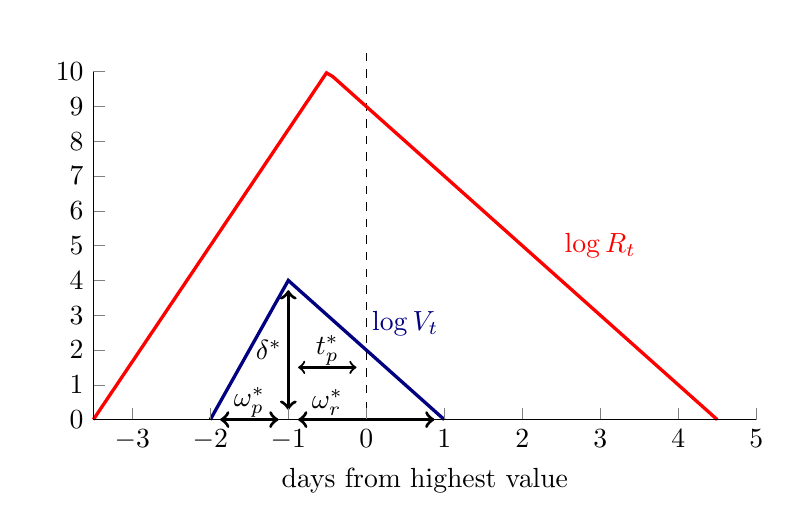
\begin{tikzpicture}
            \begin{axis}[
              no markers, domain=-3.5:4.5, samples=100,
              axis lines*=left, xlabel=days from highest value, ylabel=$ $,
              height=6cm, width=10cm,
              xtick={-5,-4,-3,-2,-1,0,1,2,3,4,5}, ytick={0,1,2,3,4,5,6,7,8,9,10},
              ymin = 0, ymax = 10, xmin =-3.5, xmax = 5,
              enlargelimits=false, clip=false, axis on top,
              grid = none, name=onset,
              declare function={
                pefunc(\x)=(\x <= -0.5) * (10 / 3 * (\x + 3.5))  +
                 (\x > -0.5) * (10 - 10 / 5 * (\x + 0.5));
                pefunc2(\x)=(\x <= -1) * (4 / 1 * (\x + 2))  +
                 (\x > -1) * (4 - 4 / 2 * (\x + 1));
              }
              ]
              % \addplot [draw=none, fill=blue!20] {lnormal(1.75,0.33)}\closedcycle;
              % \addplot [very thick, blue!50!black] {lnormal(1.75,0.33)};
            %   \addplot [draw=none, fill=orange!20] {gammapdf(4, 1)}\closedcycle;
            %   \addplot [very thick, orange!50!black] {gammapdf(4, 1)};
           
              \node (a) at (axis cs: -0.5,0) { };
              \node (a0) at (axis cs: -1,0) { };
              \node (b) at (axis cs: -1,4) { };
              \node (c) at (axis cs: -0.5,10) { };
              \node (d) at (axis cs: -2,0) { };
              \node (e) at (axis cs: 1,0) { };
              \node (f) at (axis cs: -3.5,0) { };
              \node (g) at (axis cs: 4.5,0) { };
              \node (h) at (axis cs: 0,0) { };
              \node (i) at (axis cs: 0,11) { };
              \node (j) at (axis cs: -1,1.5) { };
              \node (k) at (axis cs: 0,1.5) { };
              \draw[<->, very thick](a0)--(b);
              % \draw[<->, very thick](a)--(c);
              \draw[<->, very thick](a0)--(d);
              \draw[<->, very thick](a0)--(e);
              % \draw[<->, very thick](a)--(f);
              % \draw[<->, very thick](a)--(g);
               \draw[-, dashed](h)--(i);
              \draw[<->, thick](j)--(k);
              \node at (axis cs: -0.5,0.5) {$\omega^*_r$};
              % \node at (axis cs: 2,0.5) {$\omega_r$};
              \node at (axis cs: -1.5,0.5) {$\omega^*_p$};
              \node at (axis cs: -0.5,2) {$t^*_p$};
              % \node at (axis cs: -2.5,0.5) {$\omega_p$};
              \node at (axis cs: -1.25,2) {$\delta^*$};
              % \node at (axis cs: -0.75,6) {$\delta$};
              \addplot [very thick, red] {pefunc(x)};
              \addplot [very thick, blue!50!black, domain =-2:1] {pefunc2(x)};
              \node[red] at (axis cs: 3,5) {$\log R_t$};
              \node[blue!50!black] at (axis cs: 0.5,2.75) {$\log V_t$};
            \end{axis}
        \end{tikzpicture}
        \label{fig:illustration2}
    \end{figure}
    
\section{Computation}

\section{Model checking and inference}

\section{Results}

\subsection{Predicting individual trajectories}

\subsection{Determining optimal quarantine or isolation policies}

There are two key determinants of whether an isolation policy will be effective: 1) can infected individuals be identified early in the infectious phase and 2) once identified how long must they remain isolated. Both can be informed by a proper model. 

\begin{figure}[p]
    \centering
    \includegraphics[width=\linewidth]{../3_figures/probability.png}
    \caption{}
\end{figure}

\begin{figure}[p]
    \centering
    \includegraphics[width=\linewidth]{../3_figures/probability_by_rapid_result.png}
    \caption{}
\end{figure}

\subsection{Inferring population parameters}

\subsection{Parameterizing transmission models}



\section{Discussion}

% \printbibliography

\clearpage

\begin{appendix}

    \renewcommand{\thefigure}{A\arabic{figure}}
    \setcounter{figure}{0}
    
    \renewcommand{\thetable}{A\arabic{table}}
    \setcounter{table}{0}
    
    \renewcommand{\theequation}{A\arabic{equation}}
    \setcounter{equation}{0}

%    \appendixwithtoc
    \newpage
    \begin{table}[p]
        \centering
        \caption{Posterior estimates of peak value.}
        \begin{tabular}{lccc}
        \toprule
         & \multicolumn{2}{c}{Peak value} \\
        Characteristic & $\exp(\beta)$ & 95\% CrI\\
        \midrule
         Age: [30,50) & 1.01 & (0.99, 1.02)\\
         Age: [50,100) & 1.00 & (0.98, 1.02)\\
         Recurrence & 0.95 & (0.92, 0.97)\\
         Variant: Alpha & 1.02 & (0.98, 1.06)\\
         Variant: Delta & 1.17 & (1.13, 1.21)\\
         Variant: Omicron & 1.05 & (1.02, 1.08)\\
         Variant: BA.4/BA.5 & 1.15 & (1.10, 1.21)\\
         Variant: other & 0.98 & (0.95, 1.02)\\
         History: Vaccinated boosted & 0.84 & (0.81, 0.87)\\
         History: Vaccinated unboosted & 0.86 & (0.83, 0.89)\\
         History: Vaccinated unreported & 0.83 & (0.80, 0.87)\\
         History: Unreported & 0.86 & (0.82, 0.91)\\
         History: Boosted unreported primary & 0.88 & (0.85, 0.90)\\
         \midrule
         Reference value, log [RNA] per ml & 17.22 & (16.81, 17.65)\\
         \bottomrule
        \end{tabular}
    \end{table}
    \begin{table}[p]
        \caption{Posterior estimates of proliferation phase duration.}
        \centering
        \begin{tabular}{lcc}
         \toprule
         & \multicolumn{2}{c}{Proliferation duration } \\
         Characteristic & $\exp(\beta)$ & 95\% CrI\\
         \midrule
         Age: [30,50) & 0.97 & (0.91, 1.04)\\
         Age: [50,100) & 1.08 & (0.99, 1.19)\\
         Recurrence & 0.86 & (0.77, 0.95)\\
         Variant: Alpha & 0.79 & (0.68, 0.91)\\
         Variant: Delta & 0.66 & (0.57, 0.75)\\
         Variant: Omicron & 0.93 & (0.82, 1.04)\\
         Variant: BA.4/BA.5 & 0.87 & (0.68, 1.14)\\
         Variant: other & 1.11 & (0.97, 1.26)\\
         History: Vaccinated boosted & 1.44 & (1.27, 1.64)\\
         History: Vaccinated unboosted & 1.17 & (1.02, 1.35)\\
         History: Vaccinated unreported & 1.22 & (1.03, 1.45)\\
         History: Unreported & 1.14 & (0.94, 1.39)\\
         History: Boosted unreported primary & 1.32 & (1.17, 1.50)\\
         \midrule
         Reference value, days & 7.29 & (6.61, 8.04)\\
         Reference value (lod), days & 4.67 & (4.23, 5.15)\\
         \bottomrule
         \end{tabular}
   \end{table}

 \begin{table}[p]
    \centering
    \caption{Posterior estimates of clearance phase duration.}
    \begin{tabular}{lcc}
     \toprule
     & \multicolumn{2}{c}{Clearance duration} \\
     Characteristic & $\exp(\beta)$ & 95\% CrI\\
     \midrule
     Age: [30,50) & 1.04 & (1.01, 1.08)\\
     Age: [50,100) & 1.19 & (1.13, 1.26)\\
     Recurrence & 0.74 & (0.70, 0.79)\\
     Variant: Alpha & 0.95 & (0.87, 1.04)\\
     Variant: Delta & 0.92 & (0.85, 1.00)\\
     Variant: Omicron & 0.90 & (0.84, 0.96)\\
     Variant: BA.4/BA.5 & 0.87 & (0.78, 0.97)\\
     Variant: other & 1.02 & (0.94, 1.10)\\
     History: Vaccinated boosted & 0.86 & (0.80, 0.93)\\
     History: Vaccinated unboosted & 0.74 & (0.68, 0.81)\\
     History: Vaccinated unreported & 0.79 & (0.72, 0.87)\\
     History: Unreported & 0.98 & (0.88, 1.10)\\
     History: Boosted unreported primary & 0.87 & (0.81, 0.93)\\
     \midrule
     Reference value, days & 14.55 & (13.69, 15.44)\\
     Reference value (lod), days & 9.31 & (7.96, 8.71)\\
     \bottomrule
     \end{tabular}
\end{table}

\begin{table}[p]
    \centering
    \caption{Correlation between [RNA] and viral culture}
    \begin{tabular}{lcccc}
     \toprule
     Parameter & $\exp(\rho)$ & 95\% CrI & $\theta$ & 95\% CrI\\
     \midrule
     Peak ($\delta^*$) & 0.47 & (0.45, 0.50) &  & \\
     Proliferation ($\omega_p^*$) & 0.50 & (0.43, 0.59) &  & \\
     Clearance ($\omega_r^*$) & 0.38 & (0.35, 0.42) &  & \\
     \midrule
     Peak time ($t_p^*$) & 1.37 & (1.15, 1.64) & -0.05 & (-0.32, 0.24)\\
     \bottomrule
     \end{tabular}
    \label{tab:corr}
\end{table}

\begin{table}[p]
    \centering
    \caption{LFD positivity as a function of [RNA] and viral culture}
    \begin{tabular}{lcc}
     \toprule
     Predictor & $\exp(\gamma)$ & 95\% CrI\\
     \midrule
     log RNA copies & 1.60 & (1.41, 1.80)\\
     log PFU culturable virus & 1.27 & (1.12, 1.45)\\
     \midrule
     Intercept & -6.41 & (-7.80, -5.00)\\
     \bottomrule
     \end{tabular}
    \label{tab:lfd}
\end{table}
\end{appendix}


\end{document}